\documentclass[11pt,a4paper,notitlepage]{report}
% Shared preamble for the raw chapter-4 write-ups under docs/report/insights/.
%
% Each experiment_N/experiment_N.tex is a standalone, compilable LaTeX report
% written BEFORE anything goes into final_report/chapters/chapter_4_*.tex.
% It uses the final report's fonts, units and macros so that passages, tables
% and figures lift into the chapter without reformatting.
%
%   \documentclass[11pt,a4paper]{report}
%   % Shared preamble for the raw chapter-4 write-ups under docs/report/insights/.
%
% Each experiment_N/experiment_N.tex is a standalone, compilable LaTeX report
% written BEFORE anything goes into final_report/chapters/chapter_4_*.tex.
% It uses the final report's fonts, units and macros so that passages, tables
% and figures lift into the chapter without reformatting.
%
%   \documentclass[11pt,a4paper]{report}
%   % Shared preamble for the raw chapter-4 write-ups under docs/report/insights/.
%
% Each experiment_N/experiment_N.tex is a standalone, compilable LaTeX report
% written BEFORE anything goes into final_report/chapters/chapter_4_*.tex.
% It uses the final report's fonts, units and macros so that passages, tables
% and figures lift into the chapter without reformatting.
%
%   \documentclass[11pt,a4paper]{report}
%   \input{../common/preamble}
%   \begin{document} ...
%
% Figures and tables are NOT copied: \graphicspath and \reporttable resolve into
% final_report/figures/ and final_report/tables/, so the raw write-up always
% shows the same artefacts as the chapter.  Compile with:  latexmk -pdf <file>

\usepackage[T1]{fontenc}
\usepackage[utf8]{inputenc}
\usepackage{mathptmx}
\usepackage[scaled=0.92]{helvet}
\usepackage{courier}
\usepackage[a4paper,left=30mm,right=20mm,top=25mm,bottom=25mm]{geometry}
\usepackage{microtype}
\usepackage{booktabs}
\usepackage{tabularx}
\usepackage{longtable}
\usepackage{array}
\usepackage{multirow}
\usepackage{amsmath}
\usepackage{amssymb}
\usepackage{ifthen}
\usepackage{siunitx}
\usepackage{graphicx}
\usepackage{placeins}
\usepackage{caption}
\usepackage{enumitem}
\usepackage[table]{xcolor}
\usepackage{rotating}
\PassOptionsToPackage{hyphens}{url}\usepackage{url}
\usepackage[hidelinks]{hyperref}
\usepackage[nameinlink,noabbrev]{cleveref}

\graphicspath{{../../final_report/}{../../final_report/figures/}}
% \reporttable{name} inputs final_report/tables/name.tex
\newcommand{\reporttable}[1]{\input{../../final_report/tables/#1}}

\newcommand{\repo}[1]{\texttt{\detokenize{#1}}}
\sisetup{detect-all,group-separator={,},range-phrase=--,range-units=single}
\DeclareSIUnit{\pixel}{px}
\DeclareSIUnit{\mebi}{Mi}
\captionsetup{font=small,labelfont=bf}
\setlist{nosep}
\setlength{\parskip}{4pt}
\setlength{\LTcapwidth}{\textwidth}

% ---- result-slot status (RENDERED here, unlike in the final report)
\definecolor{stcompleted}{HTML}{A5D6A7}
\definecolor{stpartial}{HTML}{FFF2CC}
\definecolor{stuntested}{HTML}{FFD8A8}
\definecolor{stblocked}{HTML}{FFCDD2}
\definecolor{stfailed}{HTML}{FFCDD2}
\definecolor{stplanned}{HTML}{E0E0E0}
\newcommand{\slotstatus}[2]{%
  \par\noindent\fcolorbox{black!40}{st#1}{\parbox{\dimexpr\textwidth-2\fboxsep-2\fboxrule}{%
    \textbf{Status: #1.}\ #2}}\par\medskip}
\newcommand{\status}[1]{\textbf{#1}}

% ---- queries: RENDERED in red here so a reader sees every open concern in place
\definecolor{flagred}{HTML}{B00000}
\newcommand{\flag}[1]{\textcolor{flagred}{#1}}
\newcommand{\moved}[1]{#1}
\newenvironment{queried}[1][Questionable]%
  {\par\addvspace{0.6ex}\begingroup\color{flagred}\noindent
   \textbf{[#1]}\ \ignorespaces}%
  {\par\endgroup\addvspace{0.6ex}}

% ---- per-block performance marks (section 4.5 diagrams)
\definecolor{perfgood}{HTML}{A5D6A7}
\definecolor{perfpoor}{HTML}{FFCDD2}
\definecolor{perfnoeffect}{HTML}{D9EAF7}
\definecolor{perfnone}{HTML}{FFF2CC}
\newcommand{\perfmark}[1]{%
  \ifthenelse{\equal{#1}{good}}{\colorbox{perfgood}{\scriptsize good}}{%
  \ifthenelse{\equal{#1}{poor}}{\colorbox{perfpoor}{\scriptsize poor}}{%
  \ifthenelse{\equal{#1}{noeffect}}{\colorbox{perfnoeffect}{\scriptsize no effect}}{%
  \colorbox{perfnone}{\scriptsize no claim}}}}}

%   \begin{document} ...
%
% Figures and tables are NOT copied: \graphicspath and \reporttable resolve into
% final_report/figures/ and final_report/tables/, so the raw write-up always
% shows the same artefacts as the chapter.  Compile with:  latexmk -pdf <file>

\usepackage[T1]{fontenc}
\usepackage[utf8]{inputenc}
\usepackage{mathptmx}
\usepackage[scaled=0.92]{helvet}
\usepackage{courier}
\usepackage[a4paper,left=30mm,right=20mm,top=25mm,bottom=25mm]{geometry}
\usepackage{microtype}
\usepackage{booktabs}
\usepackage{tabularx}
\usepackage{longtable}
\usepackage{array}
\usepackage{multirow}
\usepackage{amsmath}
\usepackage{amssymb}
\usepackage{ifthen}
\usepackage{siunitx}
\usepackage{graphicx}
\usepackage{placeins}
\usepackage{caption}
\usepackage{enumitem}
\usepackage[table]{xcolor}
\usepackage{rotating}
\PassOptionsToPackage{hyphens}{url}\usepackage{url}
\usepackage[hidelinks]{hyperref}
\usepackage[nameinlink,noabbrev]{cleveref}

\graphicspath{{../../final_report/}{../../final_report/figures/}}
% \reporttable{name} inputs final_report/tables/name.tex
\newcommand{\reporttable}[1]{\input{../../final_report/tables/#1}}

\newcommand{\repo}[1]{\texttt{\detokenize{#1}}}
\sisetup{detect-all,group-separator={,},range-phrase=--,range-units=single}
\DeclareSIUnit{\pixel}{px}
\DeclareSIUnit{\mebi}{Mi}
\captionsetup{font=small,labelfont=bf}
\setlist{nosep}
\setlength{\parskip}{4pt}
\setlength{\LTcapwidth}{\textwidth}

% ---- result-slot status (RENDERED here, unlike in the final report)
\definecolor{stcompleted}{HTML}{A5D6A7}
\definecolor{stpartial}{HTML}{FFF2CC}
\definecolor{stuntested}{HTML}{FFD8A8}
\definecolor{stblocked}{HTML}{FFCDD2}
\definecolor{stfailed}{HTML}{FFCDD2}
\definecolor{stplanned}{HTML}{E0E0E0}
\newcommand{\slotstatus}[2]{%
  \par\noindent\fcolorbox{black!40}{st#1}{\parbox{\dimexpr\textwidth-2\fboxsep-2\fboxrule}{%
    \textbf{Status: #1.}\ #2}}\par\medskip}
\newcommand{\status}[1]{\textbf{#1}}

% ---- queries: RENDERED in red here so a reader sees every open concern in place
\definecolor{flagred}{HTML}{B00000}
\newcommand{\flag}[1]{\textcolor{flagred}{#1}}
\newcommand{\moved}[1]{#1}
\newenvironment{queried}[1][Questionable]%
  {\par\addvspace{0.6ex}\begingroup\color{flagred}\noindent
   \textbf{[#1]}\ \ignorespaces}%
  {\par\endgroup\addvspace{0.6ex}}

% ---- per-block performance marks (section 4.5 diagrams)
\definecolor{perfgood}{HTML}{A5D6A7}
\definecolor{perfpoor}{HTML}{FFCDD2}
\definecolor{perfnoeffect}{HTML}{D9EAF7}
\definecolor{perfnone}{HTML}{FFF2CC}
\newcommand{\perfmark}[1]{%
  \ifthenelse{\equal{#1}{good}}{\colorbox{perfgood}{\scriptsize good}}{%
  \ifthenelse{\equal{#1}{poor}}{\colorbox{perfpoor}{\scriptsize poor}}{%
  \ifthenelse{\equal{#1}{noeffect}}{\colorbox{perfnoeffect}{\scriptsize no effect}}{%
  \colorbox{perfnone}{\scriptsize no claim}}}}}

%   \begin{document} ...
%
% Figures and tables are NOT copied: \graphicspath and \reporttable resolve into
% final_report/figures/ and final_report/tables/, so the raw write-up always
% shows the same artefacts as the chapter.  Compile with:  latexmk -pdf <file>

\usepackage[T1]{fontenc}
\usepackage[utf8]{inputenc}
\usepackage{mathptmx}
\usepackage[scaled=0.92]{helvet}
\usepackage{courier}
\usepackage[a4paper,left=30mm,right=20mm,top=25mm,bottom=25mm]{geometry}
\usepackage{microtype}
\usepackage{booktabs}
\usepackage{tabularx}
\usepackage{longtable}
\usepackage{array}
\usepackage{multirow}
\usepackage{amsmath}
\usepackage{amssymb}
\usepackage{ifthen}
\usepackage{siunitx}
\usepackage{graphicx}
\usepackage{placeins}
\usepackage{caption}
\usepackage{enumitem}
\usepackage[table]{xcolor}
\usepackage{rotating}
\PassOptionsToPackage{hyphens}{url}\usepackage{url}
\usepackage[hidelinks]{hyperref}
\usepackage[nameinlink,noabbrev]{cleveref}

\graphicspath{{../../final_report/}{../../final_report/figures/}}
% \reporttable{name} inputs final_report/tables/name.tex
\newcommand{\reporttable}[1]{\input{../../final_report/tables/#1}}

\newcommand{\repo}[1]{\texttt{\detokenize{#1}}}
\sisetup{detect-all,group-separator={,},range-phrase=--,range-units=single}
\DeclareSIUnit{\pixel}{px}
\DeclareSIUnit{\mebi}{Mi}
\captionsetup{font=small,labelfont=bf}
\setlist{nosep}
\setlength{\parskip}{4pt}
\setlength{\LTcapwidth}{\textwidth}

% ---- result-slot status (RENDERED here, unlike in the final report)
\definecolor{stcompleted}{HTML}{A5D6A7}
\definecolor{stpartial}{HTML}{FFF2CC}
\definecolor{stuntested}{HTML}{FFD8A8}
\definecolor{stblocked}{HTML}{FFCDD2}
\definecolor{stfailed}{HTML}{FFCDD2}
\definecolor{stplanned}{HTML}{E0E0E0}
\newcommand{\slotstatus}[2]{%
  \par\noindent\fcolorbox{black!40}{st#1}{\parbox{\dimexpr\textwidth-2\fboxsep-2\fboxrule}{%
    \textbf{Status: #1.}\ #2}}\par\medskip}
\newcommand{\status}[1]{\textbf{#1}}

% ---- queries: RENDERED in red here so a reader sees every open concern in place
\definecolor{flagred}{HTML}{B00000}
\newcommand{\flag}[1]{\textcolor{flagred}{#1}}
\newcommand{\moved}[1]{#1}
\newenvironment{queried}[1][Questionable]%
  {\par\addvspace{0.6ex}\begingroup\color{flagred}\noindent
   \textbf{[#1]}\ \ignorespaces}%
  {\par\endgroup\addvspace{0.6ex}}

% ---- per-block performance marks (section 4.5 diagrams)
\definecolor{perfgood}{HTML}{A5D6A7}
\definecolor{perfpoor}{HTML}{FFCDD2}
\definecolor{perfnoeffect}{HTML}{D9EAF7}
\definecolor{perfnone}{HTML}{FFF2CC}
\newcommand{\perfmark}[1]{%
  \ifthenelse{\equal{#1}{good}}{\colorbox{perfgood}{\scriptsize good}}{%
  \ifthenelse{\equal{#1}{poor}}{\colorbox{perfpoor}{\scriptsize poor}}{%
  \ifthenelse{\equal{#1}{noeffect}}{\colorbox{perfnoeffect}{\scriptsize no effect}}{%
  \colorbox{perfnone}{\scriptsize no claim}}}}}

\setcounter{chapter}{4}
\renewcommand{\thesection}{4.3.\arabic{section}}
\renewcommand{\thefigure}{4.\arabic{figure}}
\renewcommand{\thetable}{4.\arabic{table}}
\title{Experiment 3: Dense Map Reconstruction and Map-Quality Evaluation\\
       \large Raw write-up for Chapter 4, Section 4.3}
\author{Bolton Athit Davies}
\date{Reporting cutoff: 26 October 2026}
\begin{document}
\maketitle

\noindent\textbf{Purpose of this document.} This is the raw, complete write-up
of Experiment 3, written before the thesis chapter; Section 4.3 of the final
report is extracted from it. Every number traces to a file under \repo{output/},
\repo{map/} or \repo{dataset/} named in the ``Reporting rules'' paragraph of its
slot. Open concerns are set in red where they arise.

% =====================================================================
\section{Simulation}
\label{sec:map-sim}

\slotstatus{partial}{Five databases are scored for geometry and drivability:
the tiny warehouse, which passes, and four realistic-warehouse maps --- two
mapping recordings, one per layout, each built closure-free under two
back-end configurations, A and B --- all of which fail the quality
criterion fixed before scoring. The tiny map's independent drivability
reference remains lost.}

\paragraph{Objective.} Verify that the reconstructed map reflects the physical
environment and is usable by a route planner.

\paragraph{Process.} RTAB-Map 0.23.7 built a database from a mapping run. The
occupancy grid was seated in world coordinates by one rigid transform measured
from the map's own occupied cells against the world file, without odometry or
ground truth. Geometry was then scored against the world's collision meshes, and
drivability by stamping the true nav2 footprint along a ground-truth route.

\paragraph{Datasets.} \Cref{tab:map-datasets} lists the tiny-warehouse
recordings and \cref{tab:map-datasets-realistic} the realistic-warehouse ones.
The tiny map's drivability reference is a separate run that no longer exists in
either storage location; the only surviving recording of the tiny warehouse is
the one that built the map. Each realistic map is probed with a recording that
did not build it.

\begin{table}[htbp]
\centering
\caption[Recordings of Experiment 3.]{Recordings of Experiment 3. Durations are
rosbag wall-clock recording durations from the dataset registry; the simulator
ran below real time.}
\label{tab:map-datasets}
\small
\begin{tabularx}{\textwidth}{>{\raggedright\arraybackslash}p{0.34\textwidth}lrr>{\raggedright\arraybackslash}X}
\toprule
Recording & World & Dur.\ (s) & Messages & Role \\
\midrule
\repo{dataset_map_tiny} & tiny, static & 63.3 & 82\,555 & built \repo{map/map_tiny.db}; substitute drivability route \\
\repo{dataset_static_tiny_repeat} & tiny, static & -- & \num{2973} poses & independent drivability route; \textbf{lost} \\
\repo{dataset_map_01} & large, static & 193.5 & 152\,291 & large-warehouse mapping run; unscored \\
\bottomrule
\end{tabularx}
\end{table}

\begin{table}[htbp]
\centering
\caption[Realistic-warehouse recordings of Experiment 3.]{Realistic-warehouse
recordings of Experiment 3, all prefixed \repo{dataset_allsensor_}. Build
recordings are on the removable drive; their span is the stamp range of the
stored nodes. Probe recordings are the static
twins listed in the recordings table of the realistic-world note, read from the
bags. U and I are the two layouts described there and in Chapter 3.}
\label{tab:map-datasets-realistic}
\small
\setlength{\tabcolsep}{4pt}
\begin{tabularx}{\textwidth}{>{\raggedright\arraybackslash}p{0.33\textwidth}lrr>{\raggedright\arraybackslash}X}
\toprule
Recording & World & Span (s) & Truth & Role \\
\midrule
\repo{realistic_map} & U, static & 285.7 & 14\,411 & formerly \repo{_mapv2}; built U-A and U-B \\
\repo{realistic_01_map} & I, static & 314.9 & 15\,760 & built I-A and I-B \\
\repo{realistic_000} & U, static & 125.5 & 6\,278 & independent probe, \SI{171.3}{\metre} \\
\repo{realistic_001} & I, static & 96.9 & 4\,847 & independent probe, \SI{133.0}{\metre} \\
\bottomrule
\end{tabularx}
\end{table}

\paragraph{Reporting rules.} The map under test is \repo{map/map_tiny.db},
created 8 September 2026 from
\path{small_warehouse_static/small_warehouse_static_tinymap.world}. The
reference occupancy was rasterised from the world file's collision geometry at
\SI{0.05}{\metre} per cell; the fitted placement is
$(1.850, 8.600)\,\si{\metre}$ at \SI{-89.90}{\degree}, measured once by
\repo{script/fit_map_pose.py}. Occupied-cell precision is the share of
occupied map cells within \SI{0.25}{\metre} of true structure; recall is the
share of true \emph{surface} cells within tolerance of an occupied cell, over
the region the map observed and over the whole building; drivability stamps the
$0.83\times0.50$~m footprint from \repo{nav2_ackermann.yaml} at every
ground-truth pose and counts collisions (false obstacles), unknown cells and
clearance. All of it is produced by \repo{script/validate_map.py} into
\repo{output/compare/rtab_map_vs_gt.png} (independent route) and
\repo{output/compare/rtab_map_vs_gt_selfcheck.png} (build run). The experimental
unit is one database, $n=1$.

\paragraph{Results.} The tiny map is geometrically faithful: \SI{96.6}{\percent}
of the cells it marks occupied lie on real structure.
\Cref{tab:map-geometry} gives the three geometry scores and their populations;
\cref{tab:map-drivability} gives drivability against the lost independent
route and against the build run; \cref{tab:map-graph} summarises the stored
graph. \Cref{fig:map-vs-gt} is the evaluation overlay for the independent
route and \cref{fig:map-vs-gt-selfcheck} the same database against its own
build run.

\begin{table}[htbp]
\centering
\caption{Occupied-cell geometry of \repo{map/map_tiny.db} against
\repo{small_warehouse_static_tinymap.world} at \SI{0.25}{\metre} tolerance.}
\label{tab:map-geometry}
\small
\begin{tabularx}{\textwidth}{>{\raggedright\arraybackslash}p{0.34\textwidth}r>{\raggedright\arraybackslash}X}
\toprule
Metric & Value & Population \\
\midrule
Occupied-cell precision & \SI{96.6}{\percent} & \num{11634} occupied cells \\
Recall, region the map observed & \SI{89.5}{\percent} & observed surfaces \\
Recall, whole building & \SI{67.2}{\percent} & all surfaces in the world file \\
\bottomrule
\end{tabularx}
\end{table}

\begin{table}[htbp]
\centering
\caption[Drivability of \repo{map/map_tiny.db} under the true nav2 footprint,
against two routes.]{Drivability of \repo{map/map_tiny.db} under the true
$0.83\times0.50$~m nav2 footprint, against two routes. ``Independent'' is
\repo{dataset_static_tiny_repeat}, which did not build the map and is lost.
``Build run'' is \repo{dataset/dataset_map_tiny}, the run the map was built
from. Geometry is identical in both cases because it does not depend on the
route.}
\label{tab:map-drivability}
\small
\setlength{\tabcolsep}{4pt}
\begin{tabularx}{\textwidth}{>{\raggedright\arraybackslash}p{0.30\textwidth}rr>{\raggedright\arraybackslash}X}
\toprule
Metric & Independent & Build run & Meaning \\
\midrule
Poses scored & \num{2973} & \num{3032} & \\
Clear and mapped & \SI{99.3}{\percent} & \SI{100.0}{\percent} & footprint free and observed \\
False obstacle & \SI{0.7}{\percent} & \SI{0.0}{\percent} & proven error \\
Unmapped under footprint & \SI{0.0}{\percent} & \SI{0.0}{\percent} & blind cells on the route \\
Clearance, median & \SI{1.07}{\metre} & \SI{1.01}{\metre} & to nearest obstacle \\
Clearance, 5th percentile & \SI{0.45}{\metre} & \SI{0.46}{\metre} & inflation radius is \SI{0.80}{\metre} \\
\bottomrule
\end{tabularx}
\end{table}

\begin{table}[htbp]
\centering
\caption[Stored contents of \repo{map/map_tiny.db}.]{Stored contents of
\repo{map/map_tiny.db}, read in read-only mode. Link rows are stored per
direction; the undirected count is the number of distinct node pairs.}
\label{tab:map-graph}
\small
\begin{tabularx}{\textwidth}{>{\raggedright\arraybackslash}p{0.30\textwidth}rr>{\raggedright\arraybackslash}X}
\toprule
Element & Rows & Undirected & Note \\
\midrule
Nodes & 30 & -- & ids 1--30, stamp span \SI{59.3}{\second} \\
Neighbour links & 56 & 28 & sequential odometry constraints \\
Global loop closures & 5 & 3 & pairs $(9,22)$, $(10,23)$, $(29,30)$ \\
Gravity links & 30 & 30 & one per node \\
Local-space links & 0 & 0 & none recorded \\
Visual words & \num{10357} & -- & vocabulary size \\
Features & \num{28374} & -- & stored keypoints \\
\bottomrule
\end{tabularx}
\end{table}

\begin{figure}[p]
  \centering
  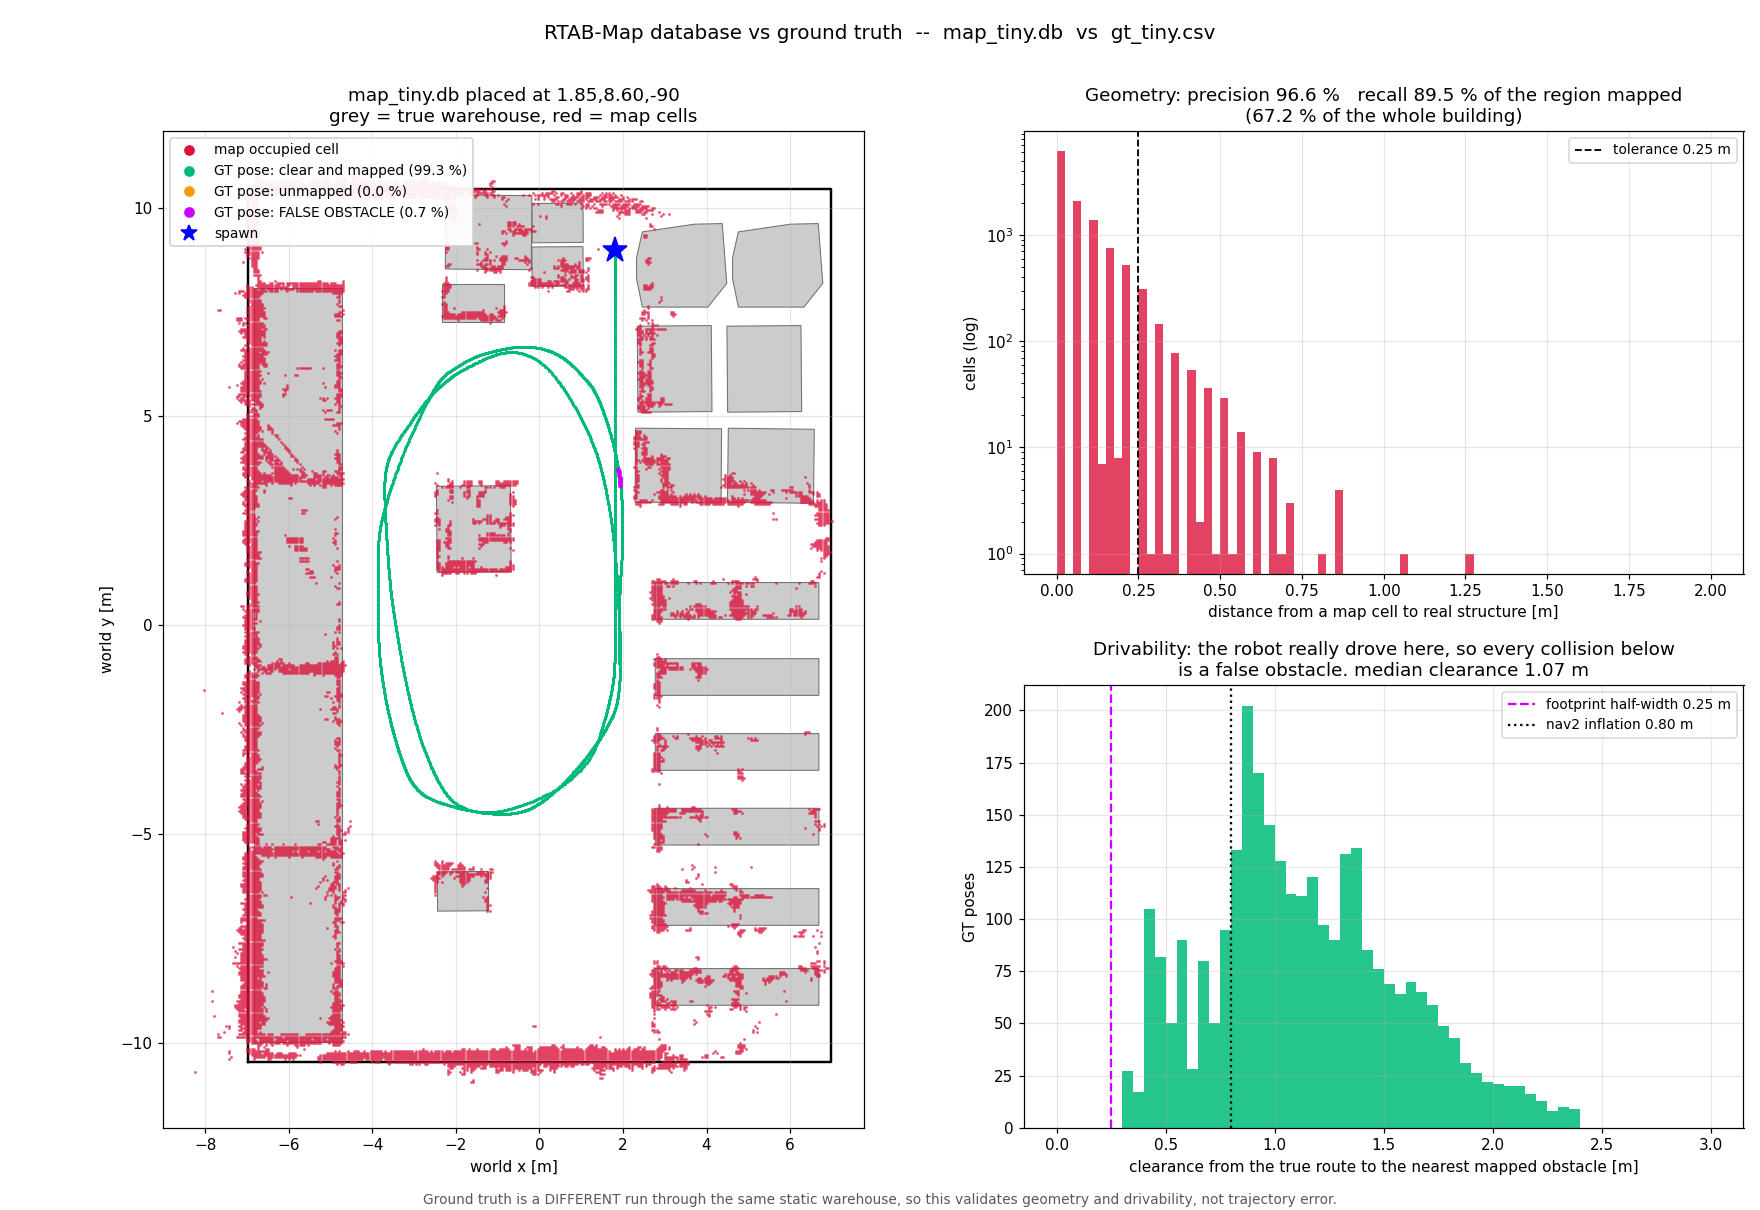
\includegraphics[width=\textwidth]{../../../output/compare/rtab_map_vs_gt.png}
  \caption[Dense-map evaluation of \repo{map/map_tiny.db} against the
  independent route.]{Dense-map evaluation of \repo{map/map_tiny.db} against
  the independent route. Left: occupied cells (red) over the world file's
  collision geometry (grey), with the ground-truth route coloured by
  drivability and the spawn marked. Top right: distance from each occupied
  cell to real structure, with the \SI{0.25}{\metre} tolerance marked. Bottom
  right: clearance from the route to the nearest mapped obstacle, against the
  footprint half-width and the nav2 inflation radius.}
  \label{fig:map-vs-gt}
\end{figure}

\begin{figure}[p]
  \centering
  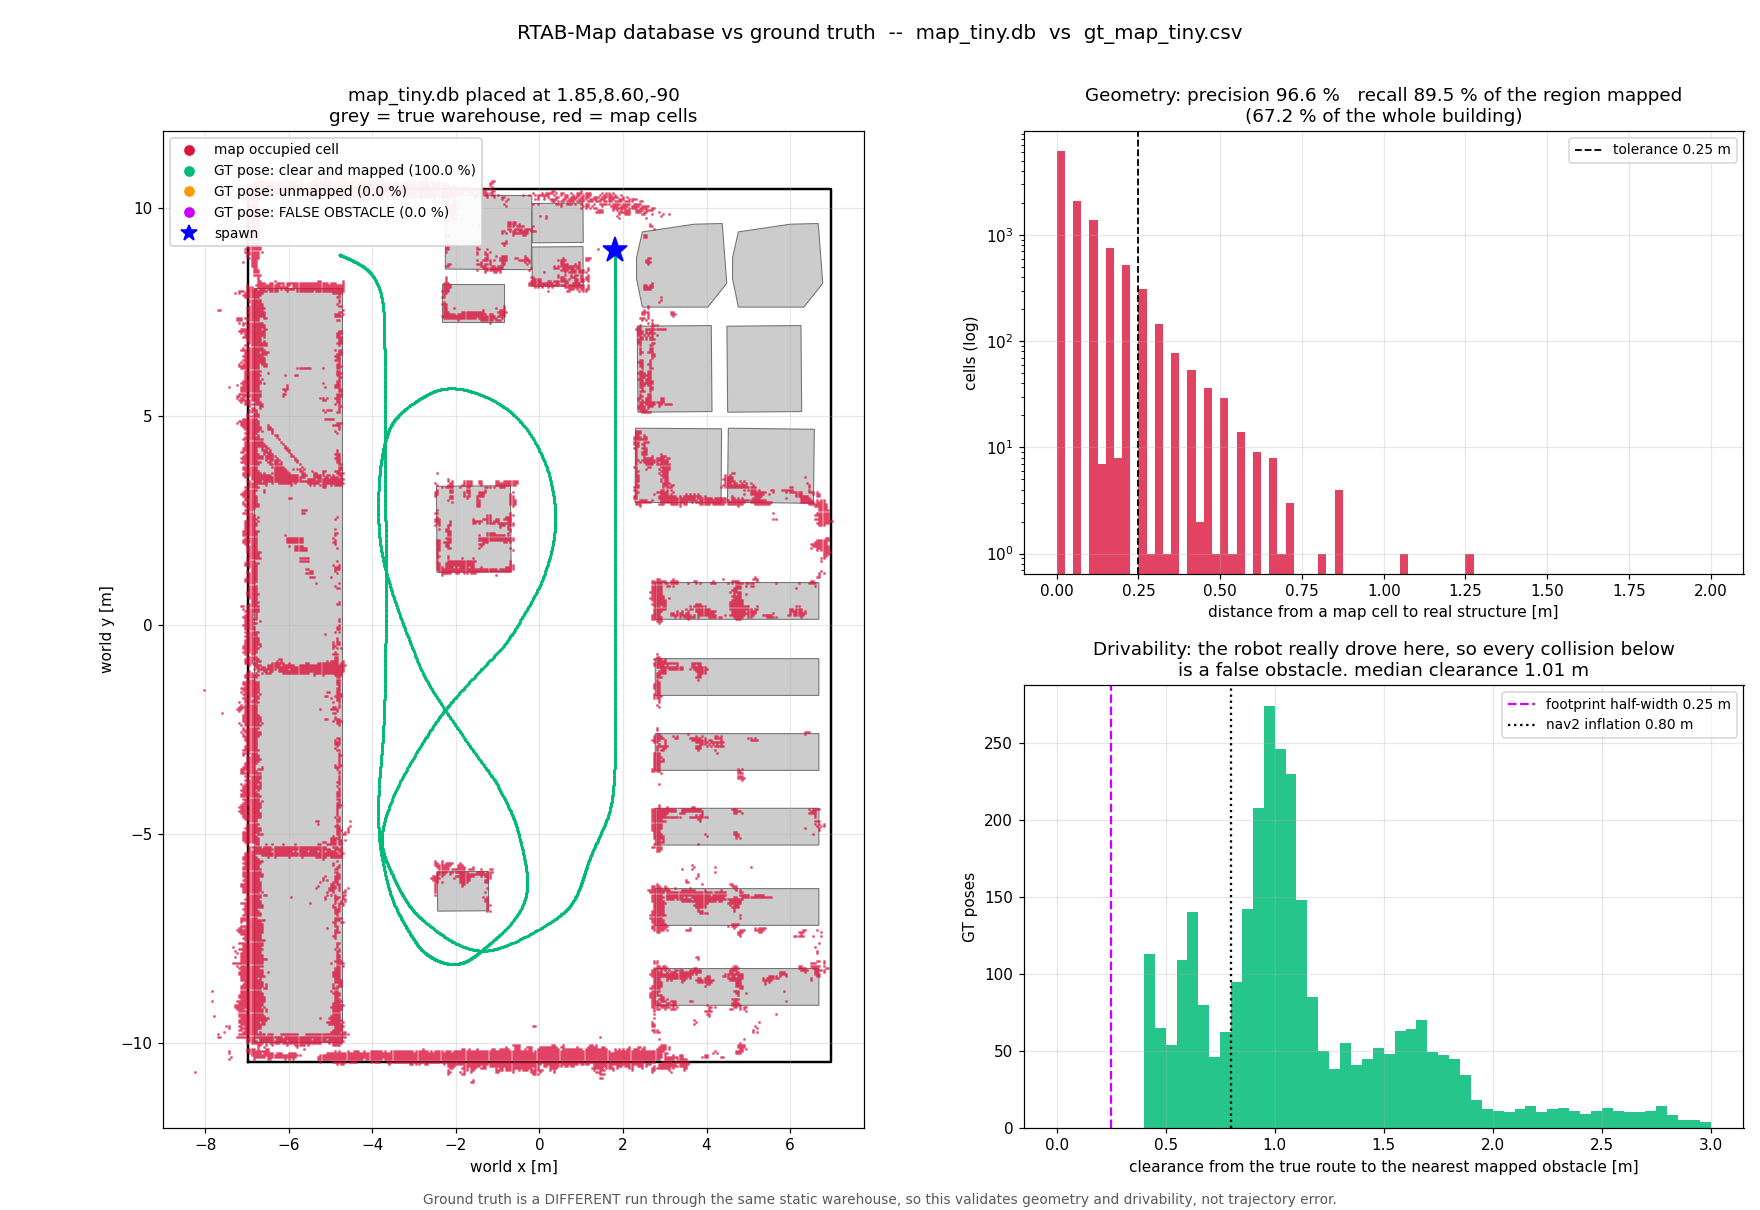
\includegraphics[width=\textwidth]{../../../output/compare/rtab_map_vs_gt_selfcheck.png}
  \caption[The same database scored against the run that built it.]{The same
  database scored against the run that built it,
  \repo{dataset/dataset_map_tiny}. The route is a figure-eight rather than the
  oval of \cref{fig:map-vs-gt}, and no pose on it collides with the map. The
  geometry panels are identical to \cref{fig:map-vs-gt}. The footer claiming a
  different run is emitted unconditionally by the evaluator and is wrong for
  this figure.}
  \label{fig:map-vs-gt-selfcheck}
\end{figure}

\paragraph{Analysis.} The gap between observed-surface recall and whole-building
recall is route coverage, not mapping failure. The run never entered the side
aisles, so about a third of the building was never seen by any sensor; the first
number describes mapping quality, the second where the robot went.

Placement is a measurement, not a tuned parameter. An independent prediction
from the spawn pose of the IMU body frame gives $(1.800, 8.662)\,\si{\metre}$,
\SI{0.080}{\metre} from the fitted value, and the fit beats the best rival
orientation more than \SI{5}{\degree} away by a \SI{60.9}{\percent} margin.
Earlier assessments that judged this database unnavigable were made with the
grid mis-seated, which is why placement is reported before any metric.

The two drivability columns measure the independence effect. Against the run
that built it the map records no false obstacle at all, because it cannot
contradict the trajectory it was constructed from; the \SI{0.7}{\percent} that
the independent route exposes is exactly what only an unseen route can reveal.
The \SI{0.0}{\percent} is a weaker question, not a better result, and is not a
map-quality figure. Three measurements show the build run is the same run: its
ground-truth poses at the stored node timestamps lie a median \SI{0.340}{\metre}
and at most \SI{0.52}{\metre} from the nodes, the nodes lie a median
\SI{0.069}{\metre} from the route in space, and all thirty nodes fall inside the
recording's sim-time interval.

Place recognition fired, but on a small graph. Two of the three closure pairs,
$(9,22)$ and $(10,23)$, join nodes about half a lap apart and are genuine
revisits; $(29,30)$ joins consecutive nodes and is not evidence of place
recognition.

Clearance couples to planner cost. The 5th-percentile clearance of
\SI{0.45}{\metre} sits below nav2's \SI{0.80}{\metre} inflation radius on both
routes, so nothing is blocked, but a planner would charge a high cost where the
robot demonstrably drove.

\textbf{Limitations, each stated once.} \emph{Lost reference:} the independent
drivability route cannot be re-read, so that half of the result is a dated
measurement. \emph{Easy route:} one loop down the wide central aisle, so
\SI{0.7}{\percent} false obstacles is a floor, not a worst case. \emph{$n=1$:}
one database on one world supports no uncertainty estimate and no claim about
the large warehouse. \emph{Residual distortion:} walls appear doubled and
thickened and shelf rows bowed in the overlay; no rigid transform removes that,
and it is the property that would limit navigation.

\begin{queried}[Queried: reproducibility of the drivability half]
The geometry result is reproducible: database and world file are both present.
The drivability result is not: \repo{dataset_static_tiny_repeat} is absent from
\repo{dataset/} and from the removable drive, the database stores an empty
parameter set so its build configuration is unrecoverable, and the RTAB-Map
engineering record's claim that the node stamps match no dataset is
contradicted by the pose agreement above. The drivability figures stand as a
dated measurement until an independent route is recorded and retained.
\end{queried}

\paragraph{Large-warehouse attempt.} The attempt \status{failed} before the
back end was exercised. The progress update of 23 September 2026 records that
the front end lost tracking in the repetitive bay structure of the large world,
the estimated pose diverged from the ground-truth route within a few time steps
of the loss, and the resulting map was not scorable; the cause was attributed to
the front end under repeated structure, not to RTAB-Map. The mapping recording
\repo{dataset_map_01} survives in the registry.
\flag{No run directory, placement fit, score or figure for this attempt is
registered, so the result rests on the progress record alone and cannot be
audited.}

\begin{queried}[Resolved and retired: unregistered databases]
Four further databases sat beside the tiny map until 6 November 2026
(\repo{map_01.db}, \repo{map_02.db}, \repo{map_02_vins.db},
\repo{map_03.db}, all written on 21 September). The insight analysis of
22 October identified them from their contents: two aborted two-node starts,
a second tiny-warehouse map on a different route, and an 18-node run that
left the floor along one aisle and fits no large world, the large-warehouse
attempt. All four were deleted on 6 November with the dataset decision,
unplaced and unscored, so the attempt is again without an artefact.
\end{queried}

\paragraph{Realistic-warehouse maps.} Four databases built in the realistic
worlds of Chapter 3 replace the unauditable large-warehouse attempt: two
mapping recordings, one per layout, each built twice, under two back-end configurations, A and B. Every one has a
registered build recording, a fitted placement, a score and a figure, and all
four fail the quality criterion fixed before they were scored.

\textbf{Reporting rules.} The criterion, fixed in
\repo{script/eval_realistic_maps.py} before any map was placed, is occupied-cell
precision $\ge$ \SI{90}{\percent}, observed-region recall $\ge$ \SI{85}{\percent}
and false obstacles $\le$ \SI{1}{\percent} of probe poses, each taken from the
tiny map's result; whole-building recall is reported, not tested. Placement was
measured by \repo{script/fit_map_pose.py} with the realistic spawn
$(5.250, 19.995, \SI{-90}{\degree})$ and confirmed on the overlays before
scoring. Scoring is the unchanged \repo{script/validate_map.py} at
\SI{0.25}{\metre} tolerance with the $0.83\times0.50$~m footprint, each map
probed by the static twin of its own layout, a recording that built none of
them. All four databases are closure-free (\repo{Rtabmap/LoopThr} 1.0,
\repo{RGBD/ProximityBySpace} false; \repo{loop_closure:=false}, RTAB-Map record
\S7c) and optimised with GTSAM. The two builds of each recording differ in
exactly three back-end parameters, \repo{Rtabmap/DetectionRate} 4 against
\SI{1}{\hertz}, \repo{Grid/RangeMax} 8 against \SI{10}{\metre} and
\repo{Grid/MaxGroundHeight} 0.29 against \SI{0.10}{\metre} (build A against build B), and in front-end session, which neither database records; they are
two configurations, not a repeat pair, so $n=1$ per cell and no difference
between builds is attributable to one parameter. The recording now named
\repo{dataset_allsensor_realistic_map} is the one held until 26 October as
\repo{_mapv2} (identical message counts); the original 103--316\,s mapping
recording and the 114-node database built from it were deleted that day, and
\repo{map/map_realistic} is the former \repo{map_realistic_v2}. Node stamps fix
the pairing: the U databases span 13--300\,s and the I databases 20--335\,s,
which the 125\,s and 97\,s probes cannot have produced. The November U
placement was fitted in the \SI{-180}{\degree} basin with \repo{--yaw-near},
because the global winner, \SI{4.2}{\percent} better by agreement, was the
rotational rival the overlay rejects; both candidates are in
\repo{fit_dataset_allsensor_realistic_map.log}. Every number is under the
experiment directory \repo{exp4-realistic-maps} of
\repo{output/compare/simulation}: the scores in
\repo{realistic_map_metrics.csv}, one \repo{validate_*.json} per map, the
inventory with the three parameters in \repo{map_inventory.json}, and the
placement logs.

\textbf{Results.} \Cref{tab:map-realistic-geometry} gives geometry,
\cref{tab:map-realistic-drivability} drivability against the independent
probes, and \cref{tab:map-realistic-graph} the stored graphs and the three
parameters that separate the builds.
\Cref{fig:map-realistic-fit,fig:map-realistic-nov-fit} are the placement
overlays of the two U builds and
\cref{fig:map-realistic-validate,fig:map-realistic-nov-validate,fig:map-realistic-01-validate,fig:map-realistic-01-nov-validate}
the evaluation overlays.

\begin{table}[htbp]
\centering
\caption[Occupied-cell geometry of the four realistic databases.]{Occupied-cell
geometry of the four realistic-warehouse databases
against their world files at \SI{0.25}{\metre} tolerance, beside the tiny map.
Bold marks a value below the fixed criterion.}
\label{tab:map-realistic-geometry}
\small
\setlength{\tabcolsep}{4pt}
\resizebox{\textwidth}{!}{%
\begin{tabular}{llrrrrr}
\toprule
Database & Config.\ & Nodes & Occupied & Precision & Recall & Recall \\
 & & & cells & & observed & building \\
 & & & & [\si{\percent}] & [\si{\percent}] & [\si{\percent}] \\
\midrule
\repo{map_tiny} & --- & 30 & 11\,634 & 96.6 & 89.5 & 67.2 \\
\repo{map_realistic} & A & 165 & 26728 & \textbf{81.2} & \textbf{82.5} & 55.7 \\
\repo{dataset_allsensor_realistic_map} & B & 148 & 22715 & \textbf{77.8} & \textbf{74.9} & 57.1 \\
\repo{map_realistic_01} & A & 185 & 25440 & \textbf{84.8} & \textbf{81.4} & 54.5 \\
\repo{dataset_allsensor_realistic_01_map} & B & 127 & 23255 & \textbf{82.2} & \textbf{77.1} & 55.3 \\
\bottomrule
\end{tabular}}
\end{table}

\begin{table}[htbp]
\centering
\caption[Drivability of the realistic-warehouse databases under the true nav2
footprint, against independent routes.]{Drivability of the four
realistic-warehouse databases under the true $0.83\times0.50$~m nav2
footprint, against the independent probe of each layout; U-A is
\repo{map_realistic}, U-B \repo{dataset_allsensor_realistic_map}, I-A
\repo{map_realistic_01}, I-B \repo{dataset_allsensor_realistic_01_map}. The
tiny map's independent figures were 2\,973 poses, \SI{0.7}{\percent} false
obstacles, clearance 1.07 and \SI{0.45}{\metre}; its probe was one loop of a
wide aisle, so the comparison is not route-matched.}
\label{tab:map-realistic-drivability}
\footnotesize
\setlength{\tabcolsep}{4pt}
\begin{tabular}{lrrrr}
\toprule
Metric & U-A & U-B & I-A & I-B \\
\midrule
Probe poses & 6278 & 6278 & 4847 & 4847 \\
Clear and mapped [\si{\percent}] & 96.2 & 95.0 & 94.9 & 89.5 \\
False obstacle [\si{\percent}] & \textbf{3.8} & \textbf{5.0} & \textbf{4.4} & \textbf{10.2} \\
Unmapped under footprint [\si{\percent}] & 2.4 & 1.9 & 0.7 & 0.5 \\
Clearance, median [\si{\metre}] & 1.96 & 2.00 & 2.16 & 1.98 \\
Clearance, 5th percentile [\si{\metre}] & 0.62 & 0.38 & 0.36 & 0.18 \\
\bottomrule
\end{tabular}
\end{table}

\begin{table}[htbp]
\centering
\caption[Stored contents and build parameters of the realistic-warehouse
databases.]{Stored contents and build parameters of the four
realistic-warehouse databases, read in read-only mode. The three parameter rows
are the only ones that differ between the builds of a recording. Neighbour
links are stored per direction; a ``spanning'' closure joins nodes more than
three apart and none exists, by configuration. The margin is the agreement
over the best rival more than \SI{5}{\degree} away; ``basin'' marks the
placement chosen with \repo{--yaw-near}.}
\label{tab:map-realistic-graph}
\scriptsize
\setlength{\tabcolsep}{3pt}
\resizebox{\textwidth}{!}{%
\begin{tabular}{lrrrr}
\toprule
 & U-A & U-B & I-A & I-B \\
\midrule
\repo{Rtabmap/DetectionRate} [\si{\hertz}] & 4.0 & 1.0 & 4.0 & 1.0 \\
\repo{Grid/RangeMax} [\si{\metre}] & 8.0 & 10.0 & 8.0 & 10.0 \\
\repo{Grid/MaxGroundHeight} [\si{\metre}] & 0.29 & 0.1 & 0.29 & 0.1 \\
Nodes & 165 & 148 & 185 & 127 \\
Node stamp span [\si{\second}] & 285.7 & 286.2 & 314.9 & 313.9 \\
Optimised path [\si{\metre}] & 369.5 & 364.2 & 384.7 & 372.3 \\
Neighbour links, rows & 322 & 294 & 356 & 248 \\
Closure rows / spanning $>3$ & 3 / 0 & 0 / 0 & 4 / 0 & 0 / 0 \\
Visual words & 55802 & 51539 & 63276 & 44342 \\
Database size [\si{\mega\byte}] & 417 & 462 & 438 & 377 \\
Placement $(x,y,\theta)$ & $(5.300, 19.500, \SI{-179.9}{\degree})$ & $(5.200, 19.800, \SI{-180.1}{\degree})$ & $(5.150, 20.450, \SI{179.4}{\degree})$ & $(4.950, 20.400, \SI{-179.9}{\degree})$ \\
Fit agreement, margin & 0.183, \SI{+10.1}{\percent} & 0.161, \SI{-4.2}{\percent} (basin) & 0.260, \SI{+66.1}{\percent} & 0.252, \SI{+60.2}{\percent} \\
\bottomrule
\end{tabular}}
\end{table}

\begin{figure}[p]
  \centering
  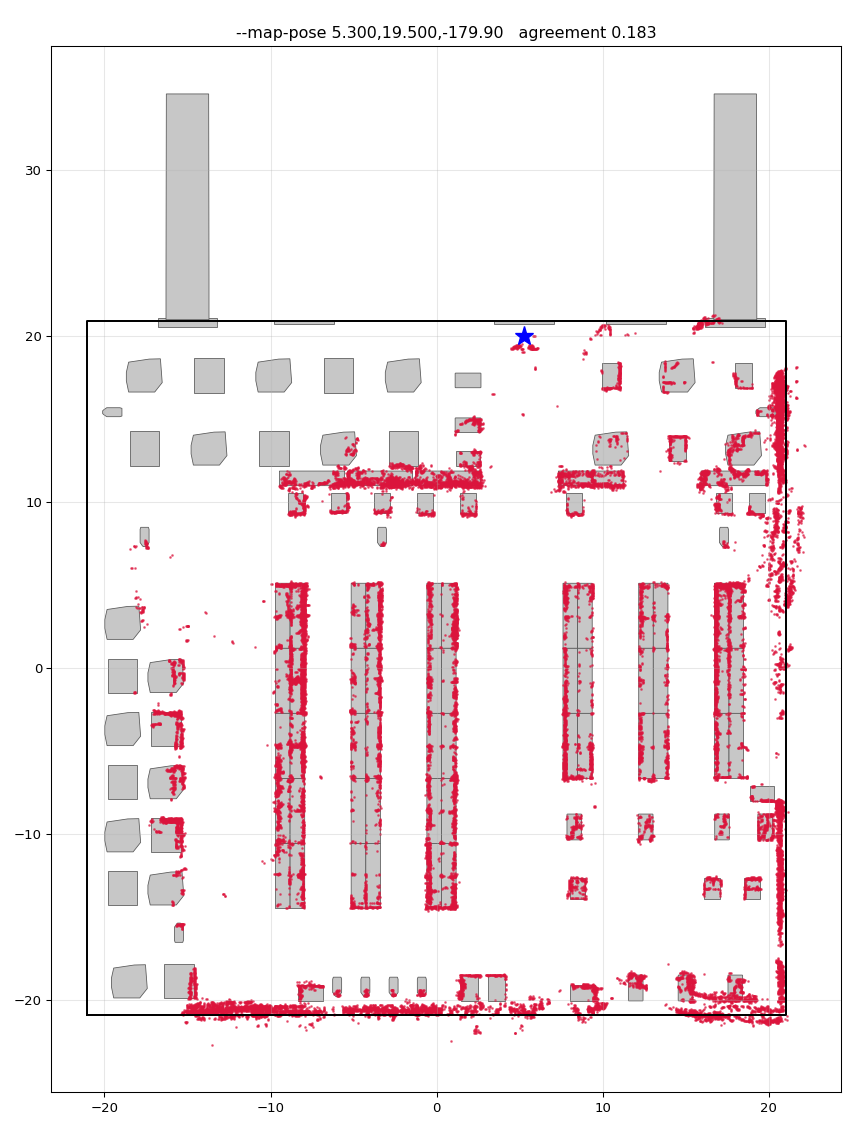
\includegraphics[width=0.7\textwidth]{figures/map_realistic_fit.png}
  \caption[Placement overlay of \repo{map/map_realistic} (U-A).]{Placement
  overlay of \repo{map/map_realistic} (U-A), agreement 0.183,
  \SI{10.1}{\percent} margin over the rival orientation. Red occupied cells
  over the world file's obstacle footprints and wall; shelf rows, the bay strip
  at $y\approx11$ and all four walls coincide.}
  \label{fig:map-realistic-fit}
\end{figure}

\begin{figure}[p]
  \centering
  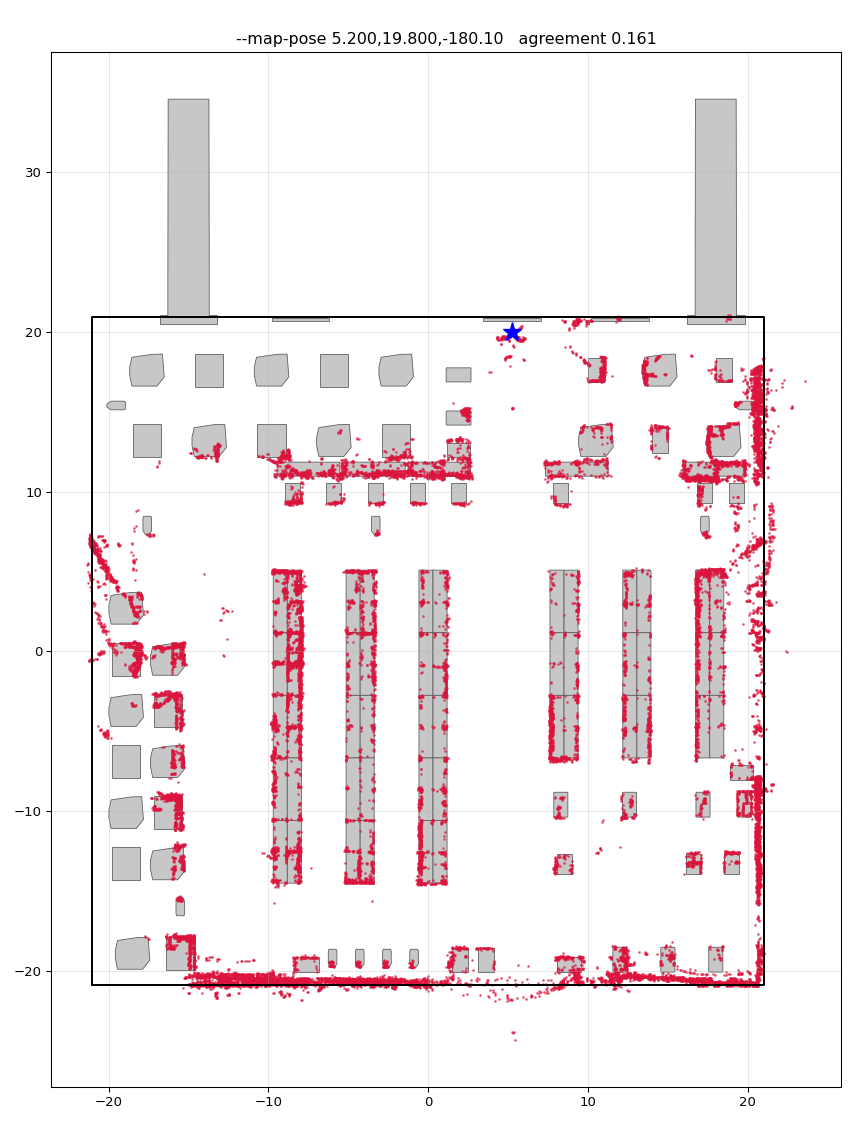
\includegraphics[width=0.7\textwidth]{figures/dataset_allsensor_realistic_map_fit.png}
  \caption[Placement overlay of \repo{map/dataset_allsensor_realistic_map}
  (U-B), fitted in the \SI{-180}{\degree} basin.]{Placement overlay of
  \repo{map/dataset_allsensor_realistic_map} (U-B). The unconstrained sweep
  preferred the \SI{180}{\degree}-rotated rival at $(-5.6, -19.6)$, agreement
  0.168 against 0.161, which puts shelf rows between shelves; the basin
  placement shown sits \SI{0.15}{\metre} from the spawn of the IMU body, as its
  build-A sibling does.}
  \label{fig:map-realistic-nov-fit}
\end{figure}

\begin{figure}[p]
  \centering
  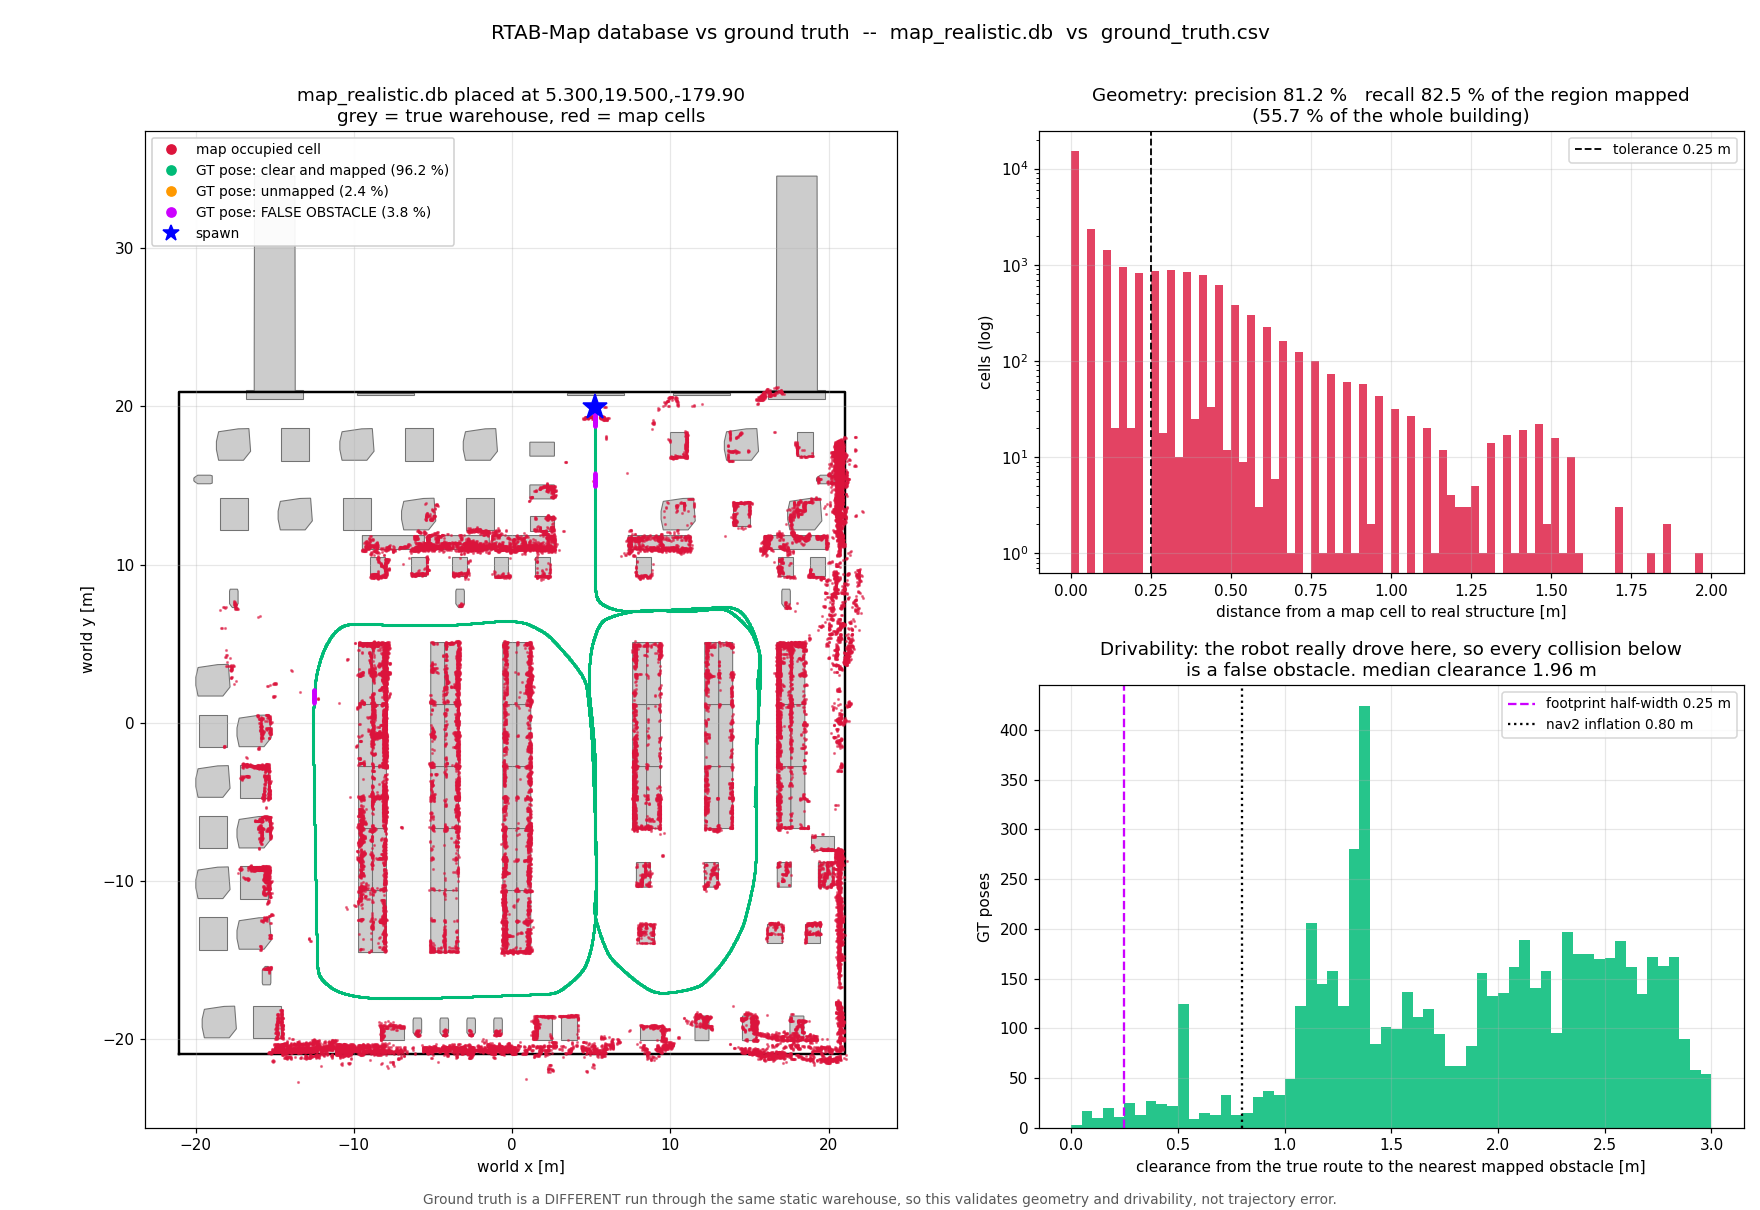
\includegraphics[width=\textwidth]{figures/map_realistic_validate.png}
  \caption[Dense-map evaluation of \repo{map/map_realistic} (U-A) against
  the independent probe.]{Dense-map evaluation of \repo{map/map_realistic}
  (U-A) against \repo{dataset_allsensor_realistic_000}. Panels as in
  \cref{fig:map-vs-gt}. The shelf rows are thickened toward the aisles; the
  false-obstacle poses sit on the first metres below the spawn and where the
  probe hugs the left shelf column at $x\approx-12.5$.}
  \label{fig:map-realistic-validate}
\end{figure}

\begin{figure}[p]
  \centering
  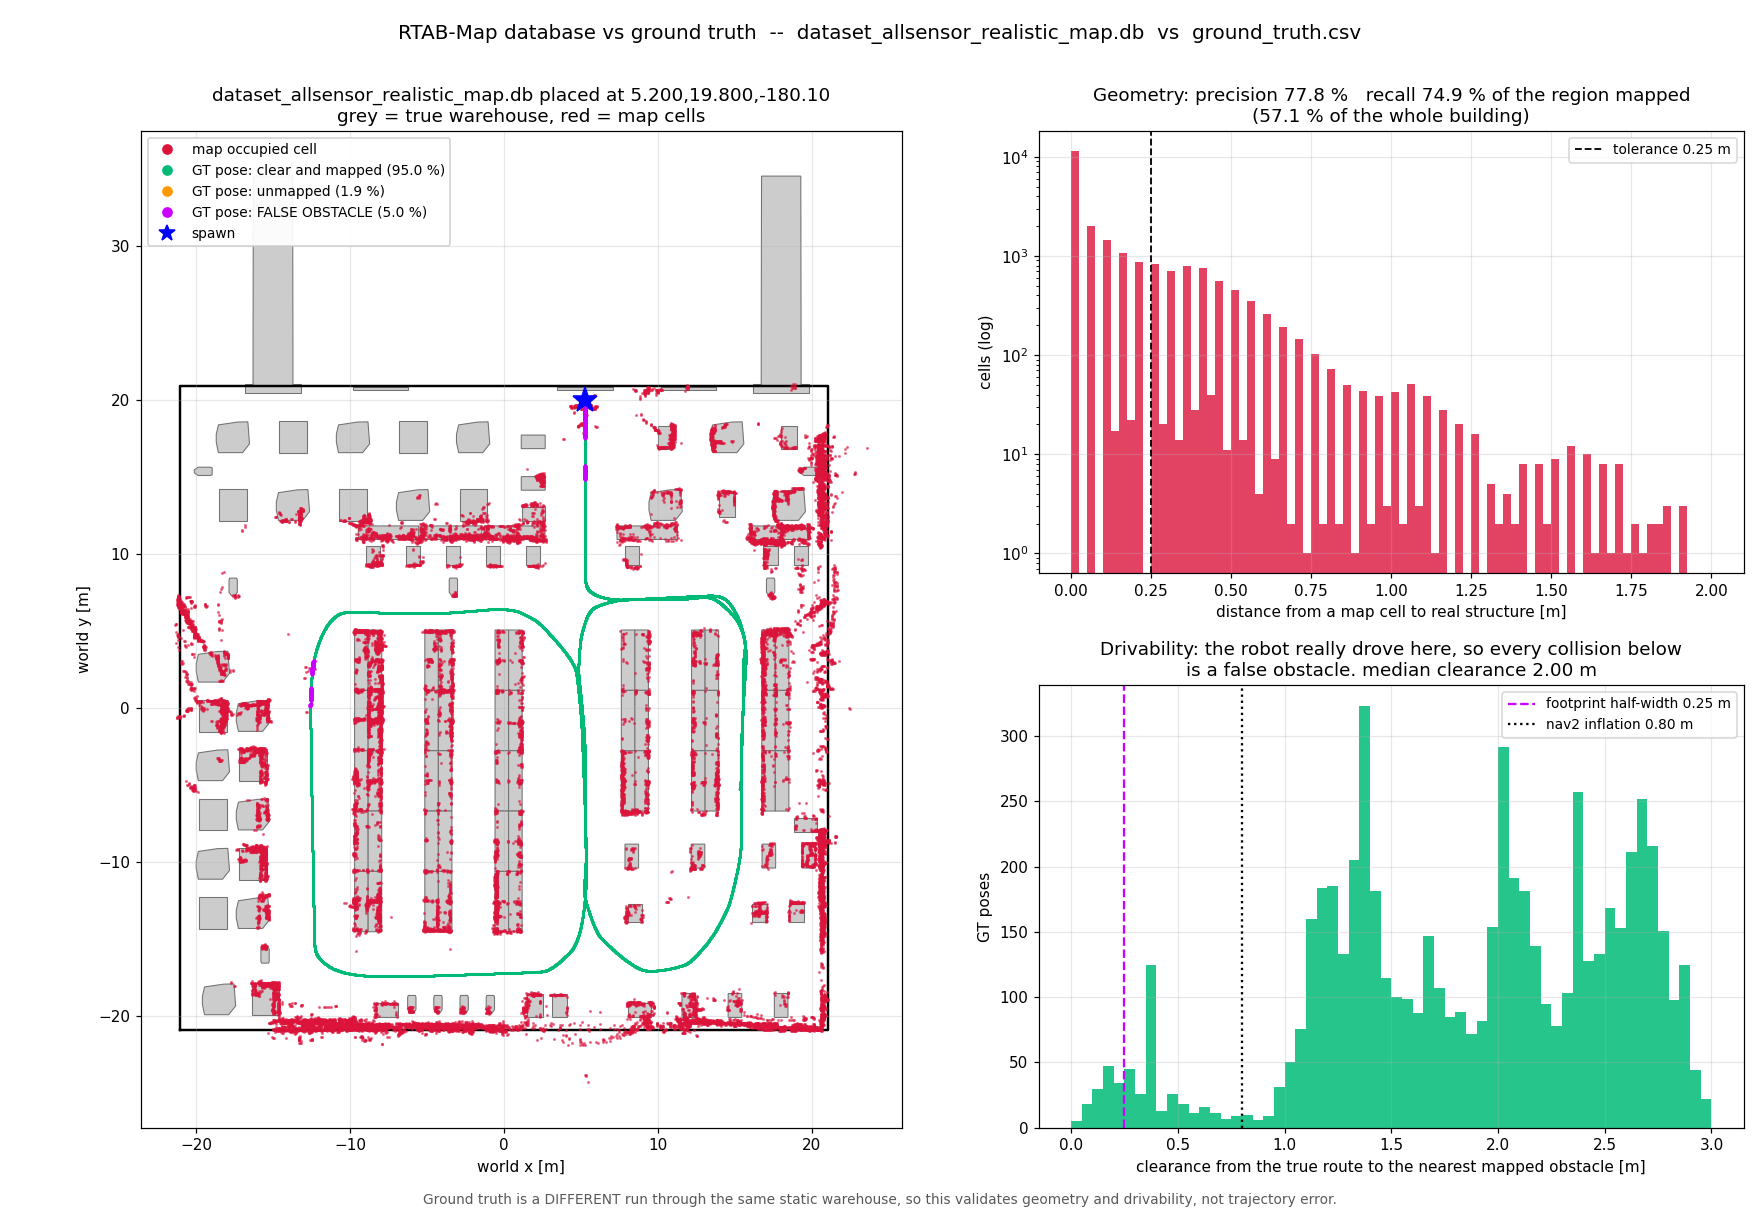
\includegraphics[width=\textwidth]{figures/dataset_allsensor_realistic_map_validate.png}
  \caption[Dense-map evaluation of \repo{map/dataset_allsensor_realistic_map}
  (U-B) against the independent probe.]{Dense-map evaluation of
  \repo{map/dataset_allsensor_realistic_map} (U-B) against the same probe.
  The same two blocked places as U-A, the spawn stretch now longer, and more
  scatter in the outer bays and along the west wall, which this build's
  \SI{10}{\metre} grid range reaches and the build A's did not.}
  \label{fig:map-realistic-nov-validate}
\end{figure}

\begin{figure}[p]
  \centering
  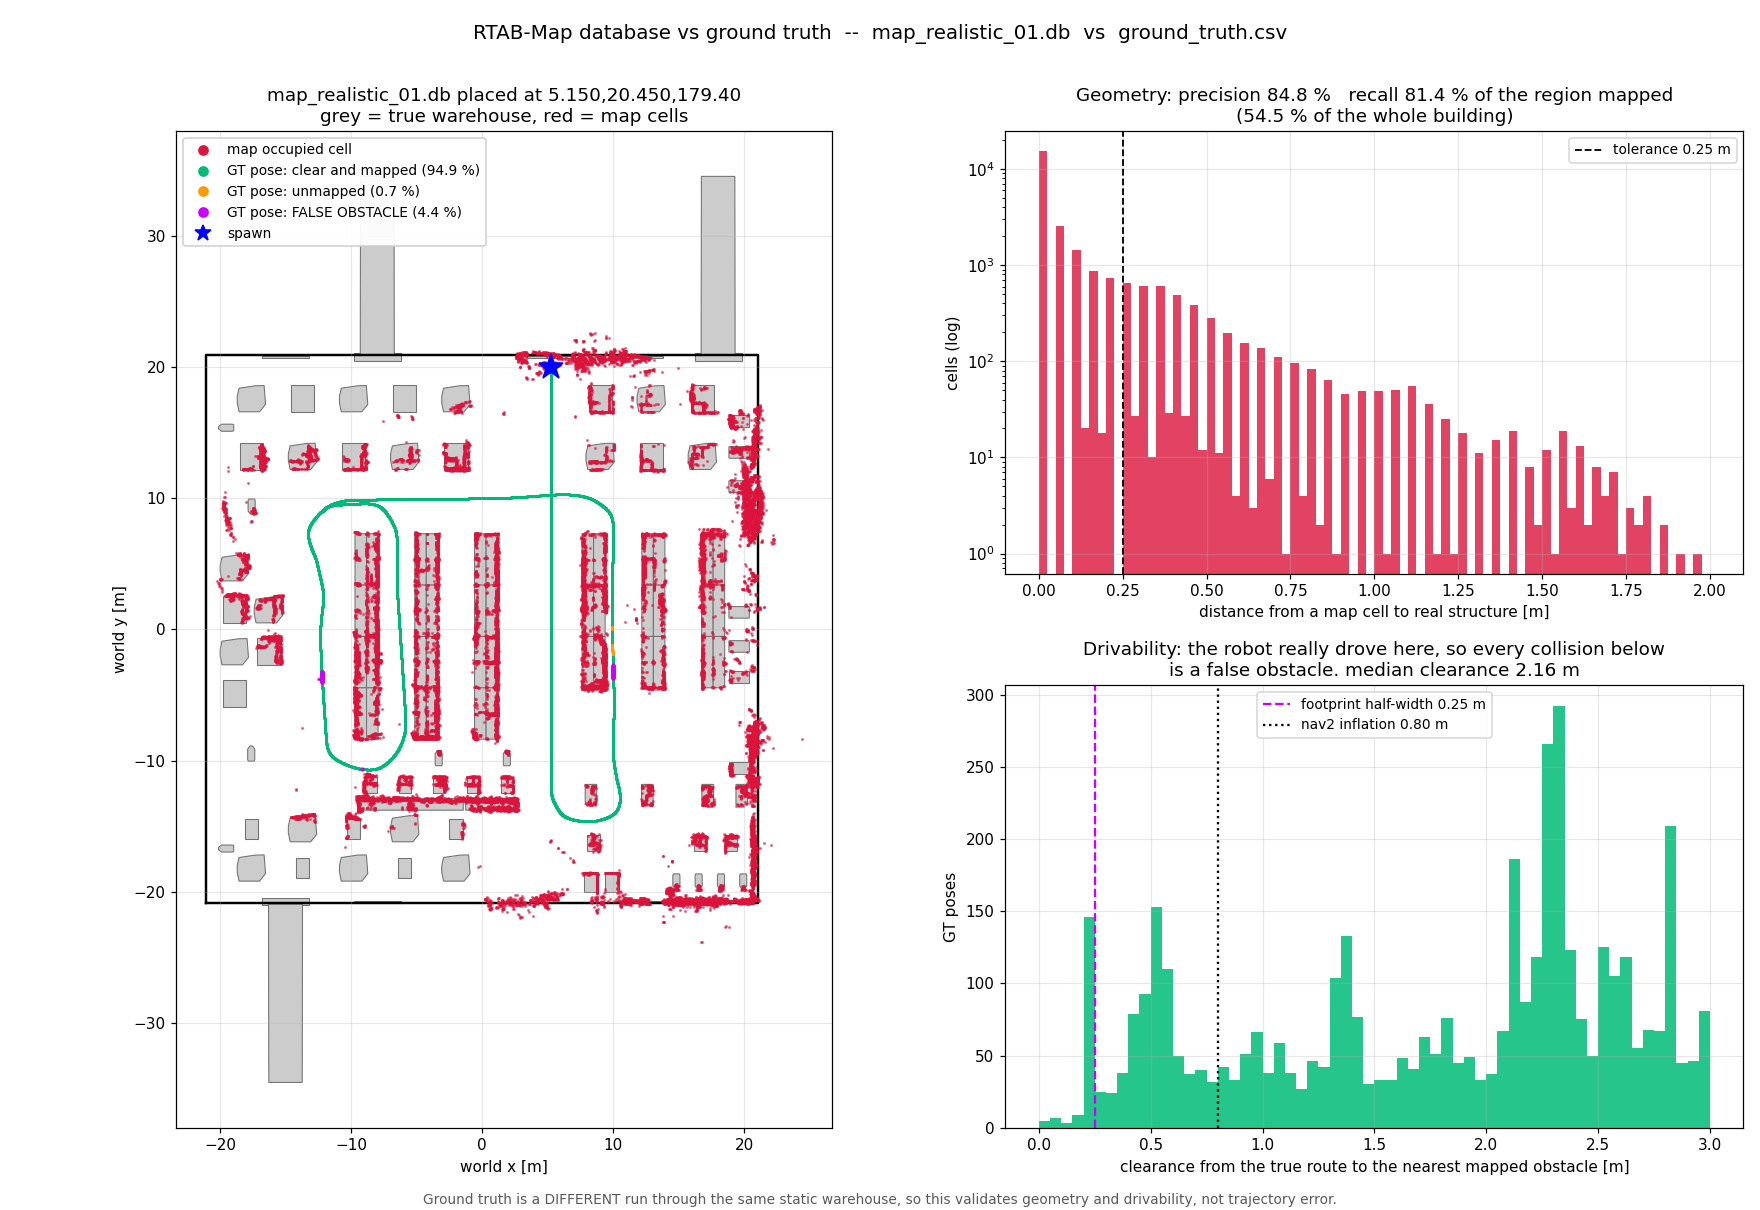
\includegraphics[width=\textwidth]{figures/map_realistic_01_validate.png}
  \caption[Dense-map evaluation of \repo{map/map_realistic_01} (I-A) against
  the independent probe.]{Dense-map evaluation of \repo{map/map_realistic_01}
  (I-A) against \repo{dataset_allsensor_realistic_001}. The clearance mode at
  exactly \SI{0.25}{\metre} is the probe threading the one-aisle gap at
  $x\approx10$ between two mapped shelf rows.}
  \label{fig:map-realistic-01-validate}
\end{figure}

\begin{figure}[p]
  \centering
  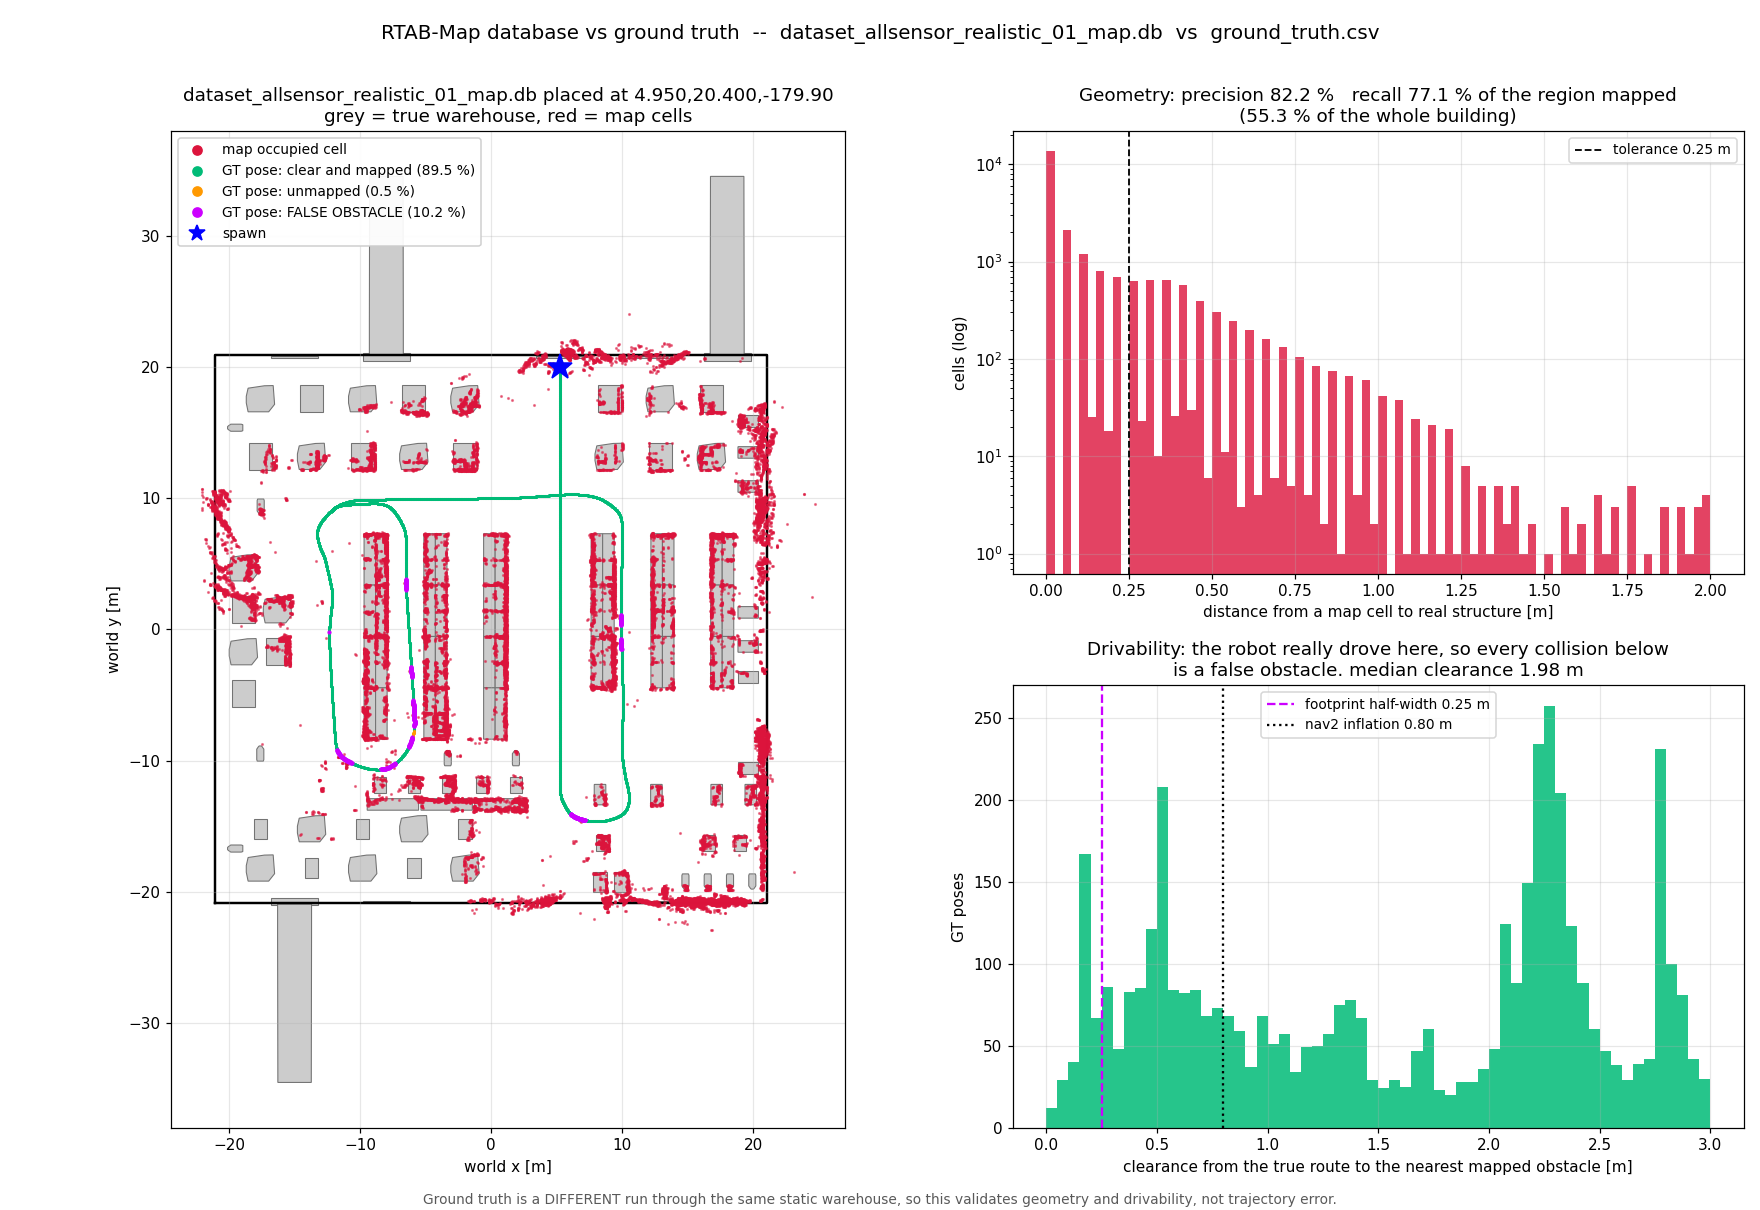
\includegraphics[width=\textwidth]{figures/dataset_allsensor_realistic_01_map_validate.png}
  \caption[Dense-map evaluation of
  \repo{map/dataset_allsensor_realistic_01_map} (I-B) against the
  independent probe.]{Dense-map evaluation of
  \repo{map/dataset_allsensor_realistic_01_map} (I-B) against the same probe.
  The blocked poses are no longer confined to the spawn: stretches of 68, 55
  and 50 poses sit mid-route in the aisles of the probe's left loop and along
  its bottom straight, on cells the map places on the floor of the aisle.}
  \label{fig:map-realistic-01-nov-validate}
\end{figure}

\textbf{Analysis.} All four maps fail, and the build B of each recording
scores below its build-A sibling on every criterion: precision by 3.4 and 2.6
points, observed recall by 7.6 and 4.3, false obstacles from 3.8 to 5.0 and
from 4.4 to \SI{10.2}{\percent}. The build-A pair fail by similar margins on
both layouts, which made their failure a property of the build rather than of
one run; the build-B pair move it further in the same direction.

Three parameters moved together between the builds, and each has its own
signature in the data, so the reading is consistent-with, not attribution. The
detection rate, 4 to \SI{1}{\hertz}, shows as fewer nodes (148 against 165, 127
against 185) and fewer observations per cell, which the view-count effect of
the tiny-map insight analysis turns into lower precision and recall. The grid
range, 8 to \SI{10}{\metre}, shows as structure the build As never
reached: the west wall and the far outer bays now carry occupied cells, and the
largest new phantom clusters sit on them. The ground-height threshold, 0.29 to
\SI{0.10}{\metre}, shows where it would: on the I layout the build B
blocks 518 probe poses against 213, and the new stretches are mid-route, in
the aisles, on cells first observed at median node 27 rather than at the
start. A one-parameter rebuild is the test that would separate the three, and
is the next action.

In the build As the loss is mostly thickened structure, with a phantom
share the tiny map did not have. Classifying the wrong cells
(\repo{script/exp4_insights.py}): 13.4 and \SI{9.7}{\percent} of occupied
cells are surfaces drawn too thick, within \SI{0.50}{\metre} of true
structure, and 5.2 and \SI{5.3}{\percent} are phantoms further out, against
3.0 and \SI{0.4}{\percent} on the tiny map; in the build Bs the shares
are 15.4 and \SI{11.5}{\percent} thickened and 7.3 and \SI{6.3}{\percent}
phantom. The thickening sits on the shelf rows the build route passed; the
phantoms are the east and south walls, drawn about \SI{0.5}{\metre} off their
true line in all four maps and far from any route. In the build As the
false obstacles are not the thickened shelving: every blocked probe pose lies
within \SI{0.6}{\metre} of a phantom cell, the largest blocked stretch of each
map is the first metres from the spawn, and 96 and \SI{63}{\percent} of the
phantom cells under those stretches were first observed by one of the first
five graph nodes, during the inertial initialisation transient. The November U
build repeats that pattern (224 spawn poses, \SI{88}{\percent} of the blocking
cells early); the November I build does not, which is the ground-height
signature above.

All four are an odometry picture by design, and should be read as one. Loop
closure was disabled on both sides of the pipeline after the A/B of 26 October
showed the front end's own closures corrupting an otherwise \SI{0.1}{\metre}
map (RTAB-Map record \S7c), so no node was ever corrected against a revisited
place; the stored graphs confirm it, with no closure spanning more than three
nodes and none at all in the build Bs. The thickening and the displaced
walls are therefore uncorrected drift along a 365--385-metre build route
re-observing the same structure from slightly different estimated places,
which is what this configuration was built to expose. It is not evidence
about RTAB-Map's loop closing, which was not exercised.

Whole-building recall of 54.5 to \SI{57.1}{\percent} is route coverage, as on
the tiny map: the build routes loop the central block and the outer bays were
seen only in passing. Observed-region recall, the mapping figure, is 74.9 to
\SI{82.5}{\percent}.

Placement needed the overlay on three of the four fits, and the spawn check
did not apply to any. The fits land about \SI{180}{\degree} from the
\SI{-90}{\degree} spawn prediction because the map frame was seated during the
inertial initialisation transient rather than at the body's spawn pose: node 1
of the October databases carries a yaw of \SI{57}{} and \SI{-89}{\degree} and a
height still settling over the first nodes, where the tiny map's node 1 is the
identity. On the November U build the unconstrained sweep chose the rotated
rival outright; the overlays leave no doubt about any of the four placements,
and the two builds of each layout agree to \SI{0.3}{\metre} and
\SI{0.5}{\degree}.

\textbf{Limitations, each stated once.} \emph{Not route-matched:} the tiny
probe was one loop of a wide aisle, these probes thread shelf aisles
(5th-percentile clearance 0.18--0.62 against \SI{0.45}{\metre}), so part of the
false-obstacle gap is probe difficulty and the \SI{1}{\percent} threshold was
set against an easier route. \emph{No attribution:} world and route vary
together between layouts, and three parameters and the front-end session vary
together between builds, so no factor may be credited for any difference in
this slot. \emph{$n$:} one database per cell supports no uncertainty estimate.
\emph{Front end unrecorded:} the databases store the back end's parameters but
not which front end, in which session, supplied the odometry chain.

\begin{queried}[Queried: front end of the realistic builds]
RTAB-Map took its pose from TF, so the odometry came from whichever front end
was running; none of the four databases records which, and the build Bs
were made during the latency sessions of Experiment~3, whose load on the front
end is not recorded either. The precision loss cannot be placed on the front
end against the back end, nor the November drop on parameters against session,
until the build manifest names both.
\end{queried}

\paragraph{Were the poses the problem?} All four maps fail, and the failure
could lie in the trajectory the grid was built along or in how the grid was
built along it. The databases do not record which front end supplied their
odometry, so the failure cannot be placed on a front end; the poses
themselves can still be measured,
because the graph is in the database and both mapping recordings have ground
truth. \Cref{tab:map-graph-accuracy} scores every node against the recording
it was built from.

The poses are not the problem. Through the same fitted placement the occupancy
grid was scored with, the graphs sit \SI{0.102}{} and
\SI{0.128}{\metre} rms from the truth on the U layout and \SI{0.396}{} and
\SI{0.331}{\metre} on the I layout, which is \SIrange{0.03}{0.10}{\percent}
of the \SIrange{365}{381}{\metre} routes, every node of all four graphs
scored. A best-fit alignment of each graph
improves it by at most \SI{0.012}{\metre}, so the placements are right as
well: these maps are neither in the wrong place nor the wrong shape. Every one
of those figures is inside the \SI{0.25}{\metre} tolerance at which the
occupancy grids were scored, so a grid built from perfect poses would have been
scored the same way.

What follows is an attribution the chapter could not make before. The
\SIrange{77.8}{84.8}{\percent} occupied-cell precision and the
\SIrange{3.8}{10.2}{\percent} false-obstacle rate are not inherited from the
trajectory; they are produced where the grid is built from the depth image ---
the sensor range, the ground-height threshold and the ray tracing of the
map-evaluation method --- and that is where a fix has to be looked for.
Two qualifications hold it in place. The I-layout graphs reach
\SI{3.207}{} and \SI{2.586}{\metre} at their worst single node against
\SI{0.412}{} and \SI{0.287}{\metre} on the U layout, so the I builds do carry
a local excursion that the rms hides and that could account for part of one
layout's loss, though not for a failure both layouts share. And a graph is
scored at its nodes, one every few metres, while the grid is written from every
frame between them; a pose error that appears and is corrected between two
nodes would not be seen here.

\reporttable{map_graph_accuracy}

\paragraph{Summary.} Where tracking holds, the mapping pipeline is
geometrically sound on the tiny map: occupied-cell precision \SI{96.6}{\percent}
and observed-surface recall \SI{89.5}{\percent}, with whole-building recall of
\SI{67.2}{\percent} explained by route coverage; the drivability half is a dated
measurement whose independent reference is lost. On the realistic warehouse
four maps built without loop closure, two per layout under back-end
configurations A and B, are auditable end to end and all fail the same
criterion: precision 77.8 to \SI{84.8}{\percent} and false obstacles 3.8 to
\SI{10.2}{\percent} against independent probes. Their loss is thickened
shelving, displaced walls and phantoms at the spawn from uncorrected drift,
which the closure-free build was configured to expose; the current
configuration scores lower on every metric, for reasons the three parameters
it changed at once do not let this slot separate. The earlier large-warehouse
attempt that lost tracking remains unauditable.

\paragraph{Future plan.} Attribute the November drop by rebuilding one
recording with a single parameter restored at a time, first the ground-height
threshold (\repo{Grid/MaxGroundHeight}), then the detection rate, and rescoring
with the unchanged evaluator. Name the front end, its
session and the three parameters in every build manifest. Use the four maps as
the odometry baseline against which a corrected map is compared: re-enable
closure with a translation bound on accepted corrections, or merge the
closure-free sub-maps through Atlas, and rescore. Discard the cells of the
first few nodes, or start the map after the inertial transient has settled,
which the data predict would remove the spawn stretch. Record the
tiny-warehouse independent route again and retain it.

% =====================================================================
\FloatBarrier
\section{Real robot}
\label{sec:map-real}

\slotstatus{planned}{No RTAB-Map database has been built from real imagery,
and no reference geometry of the site exists to score one against.}

\paragraph{Reason.} The geometry metric scores occupied cells against known
collision geometry, and the placement step needs that geometry; the mock
warehouse has no such model. The drivability metric needs a tracked route from
a run other than the mapping run. Neither input exists at the cutoff.

\paragraph{Next action.} Survey the mock warehouse (walls, stacks, walkway)
into a reference occupancy grid at \SI{0.05}{\metre}, build a database from a
real mapping run, and score it with the unchanged evaluator, using the optical
tracker route from a second run for drivability.

\end{document}
